\chapter{Analysis: Systematic uncertainties}
\label{ch:analysis-systematics}

The impact of the systematic uncertainties on the number of signal 
and background events are summarized for a LQ mass hypothesis of 500 GeV in Tables~\ref{tab:eejjSystematics} 
and~\ref{tab:enujjSystematics} for the \eejj~and \enujj~channels, respectively.
Further details on how these uncertainties are computed are given in this chapter.

\section{Background normalization} \label{sec:BkgNormUncert}
The uncertainties on the normalization factors of the main backgrounds 
are discussed in Chapter~\ref{ch:analysis-backgrounds} and summarized below:
\begin{itemize}
\item overall uncertainty on QCD multijet background in the \eejj~(\enujj) channel: \QCDUncertEEjj~(\QCDUncertEnujj)
\item scale factor for \emujj~sample for \ttbar~background estimate in \eejj~channel: \\ $\mathcal{C} = \mbox{\rescaleFactorTTBAReejj}$
\item scale factor for \ttbar~MC sample in \enujj~channel: $\mathcal{R}_{\mbox{\ttbar}} = \mbox{\rescaleFactorTTBARenujj}$
\item scale factor for \zjets~MC sample in \eejj~channel: $\mathcal{R}_{\mbox{\PZz}} = \mbox{\rescaleFactorZSherpa}$
\item scale factor for \wjets~MC samples in \enujj~channel: $\mathcal{R}_{\mbox{\PW}} = \mbox{\rescaleFactorWSherpa}$
\end{itemize}

\section{\ttbar, \zjets, and \wjets~background shape} \label{sec:BkgShapeUncert}

The systematic uncertainties due to the modeling 
of the shape of the \zjets~background (in the \eejj~channel), and  
both \ttbar~and \wjets~backgrounds (in the \enujj~channel) are determined 
by comparing the background predictions obtained with the default MC samples listed 
in Section~\ref{sec:mc-samples} with alternative {\sc MadGraph} MC samples.
These alternative {\sc MadGraph} samples have 
renormalization/factorization scales 
and jet matching thresholds varied by a factor of two. 

The number of events in the alternative MC samples is limited, and
the final \eejj~and \enujj~selection is too tight to evaluate these modeling uncertainties.
Therefore, instead of applying the full final \eejj~and \enujj~selection,
looser selection requirements are defined.  This looser selection is used to 
quantify the variation in the shapes of \mee, \st, and \mej~(for the \eejj~channel) 
and \MET, \st, and \mej~(for the \enujj~channel) between the default and the alternative samples. 
The explicit selection critera are listed in Table~\ref{tab:ResultsShapeSyst}.

The alternative samples are first normalized at either \eejj~or \enujj~preselection level to 
have the same number of events of the corresponding default samples. 
Then the additional selections reported in Table~\ref{tab:ResultsShapeSyst} 
are applied. Finally, the most significant discrepancy between the default sample 
and the alternative samples is calculated for each set of cuts considered. 
The result of this study are summarized in Table~\ref{tab:ResultsShapeSyst}. 
The distributions of the studied reconstructed quantities, for 
the default sample and for the alternative sample 
showing the most significant discrepancy, are presented 
in Figures~\ref{fig:ResultsShapeSystZJets},~\ref{fig:ResultsShapeSystWJets},~\ref{fig:ResultsShapeSystTTbar}.

This study yields the following 
systematic uncertainties on background shape:
\begin{itemize}
\item \zjets~in \eejj~channel : \BkgShapeUncerZJetsEEJJ
\item \wjets~in \enujj~channel : \BkgShapeUncerWJetsENUJJ
\item \ttbar~in \enujj~channel : \BkgShapeUncerTtbarENUJJ
\end{itemize}

\begin{table}
  \begin{center}
    \scriptsize
    \begin{tabular}{l|c|c|c|c} 
    Loose      & $N_{events}^A$ in  &  $N_{events}^D$ in  &  $(N_{events}^A / N_{events}^D) -1$ & Reference to  \\ 
    Selection & Alternative Sample &   Default Sample       &                             [\%]                                & Figure \\
    \hline	\hline
     \multicolumn{5}{c}{\zjets~in the \eejj~Channel} \\     
     \hline
     \eejj presel. $+$ \mee$>100$~\GeV & 674.05 $\pm$ 78.91 & 789.11 $\pm$ 57.68 & -14.58 $\pm$ 12.43 & \mee~(Fig.~\ref{fig:ResultsShapeSystZJets}, top)  \\
     \eejj presel. $+$ \st$>330$~\GeV & 3498.61 $\pm$ 169.77 & 3090.92 $\pm$ 131.94 & 13.19 $\pm$ 6.98  & \st~(Fig.~\ref{fig:ResultsShapeSystZJets}, middle)  \\
     \eejj presel. $+$ \mej$>60$~\GeV & 3498.61 $\pm$ 169.77 & 3090.92 $\pm$ 131.94 & 13.19 $\pm$ 6.98  & \mej~(Fig.~\ref{fig:ResultsShapeSystZJets}, bottom)  \\
    \hline	\hline
     \multicolumn{5}{c}{\wjets~in the \enujj~Channel} \\     
     \hline
     \enujj presel. $+$ \MET$>100$~\GeV & 3259.31 $\pm$ 214.76 & 3489.69 $\pm$ 283.68 & -6.60 $\pm$ 10.21 & \MET~(Fig.~\ref{fig:ResultsShapeSystWJets}, top)  \\
     \enujj presel. $+$ \st$>450$~\GeV & 2509.97 $\pm$ 224.49 & 3074.69 $\pm$ 263.94 & -18.37 $\pm$ 11.38 & \st~(Fig.~\ref{fig:ResultsShapeSystWJets}, middle)  \\
     \enujj presel. $+$ \mej$>150$~\GeV & 13270.35 $\pm$ 568.15 	& 12937.28 $\pm$ 645.48  &	 2.57 $\pm$ 6.65 & \mej (Fig.~\ref{fig:ResultsShapeSystWJets}, bottom)  \\
     \hline	\hline
     \multicolumn{5}{c}{\ttbar~in the \enujj~Channel} \\     
     \hline
     \enujj presel. $+$ \MET$>100$~\GeV & 1958.67 $\pm$ 32.58 &	 2022.04 $\pm$ 22.01 & 	 -3.13 $\pm$ 1.94 & \MET~(Fig.~\ref{fig:ResultsShapeSystTTbar}, top)  \\
     \enujj presel. $+$ \st$>450$~\GeV & 1226.93 $\pm$ 25.79 & 	 1104.13 $\pm$ 14.96  &	 11.12 $\pm$ 2.70 & \st~(Fig.~\ref{fig:ResultsShapeSystTTbar}, middle)  \\
     \enujj presel. $+$ \mej$>150$~\GeV & 4007.07 $\pm$ 46.61 &	 3919.81 $\pm$ 35.16 &	 2.23 $\pm$ 1.49 & \mej~(Fig.~\ref{fig:ResultsShapeSystTTbar}, bottom)  \\
    \end{tabular}
    \caption{Summary of the study of systematic uncertainties on background shape. 
      The "alternative sample" is the one that presents the largest deviation 
      with respect to the default sample.}
    \label{tab:ResultsShapeSyst}
  \end{center}
\end{table}


 \begin{figure}
  \begin{center}
    \begin{tabular}{cc}
      \resizebox{10cm}{!}{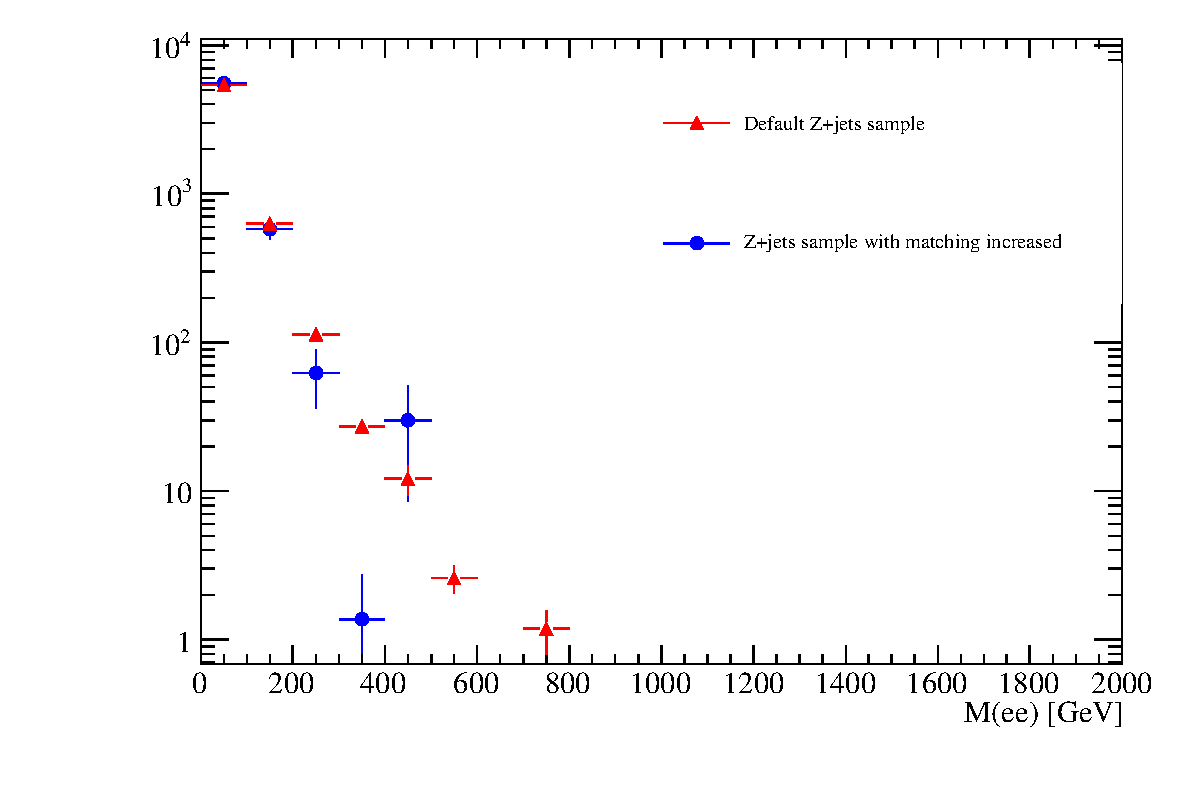
\includegraphics{tex/analysis/systematics/fig/MeeFinal_MejPresel_STPresel_ZJetsToLL_matchingup_Mee_PAS.pdf}} \\
      \resizebox{10cm}{!}{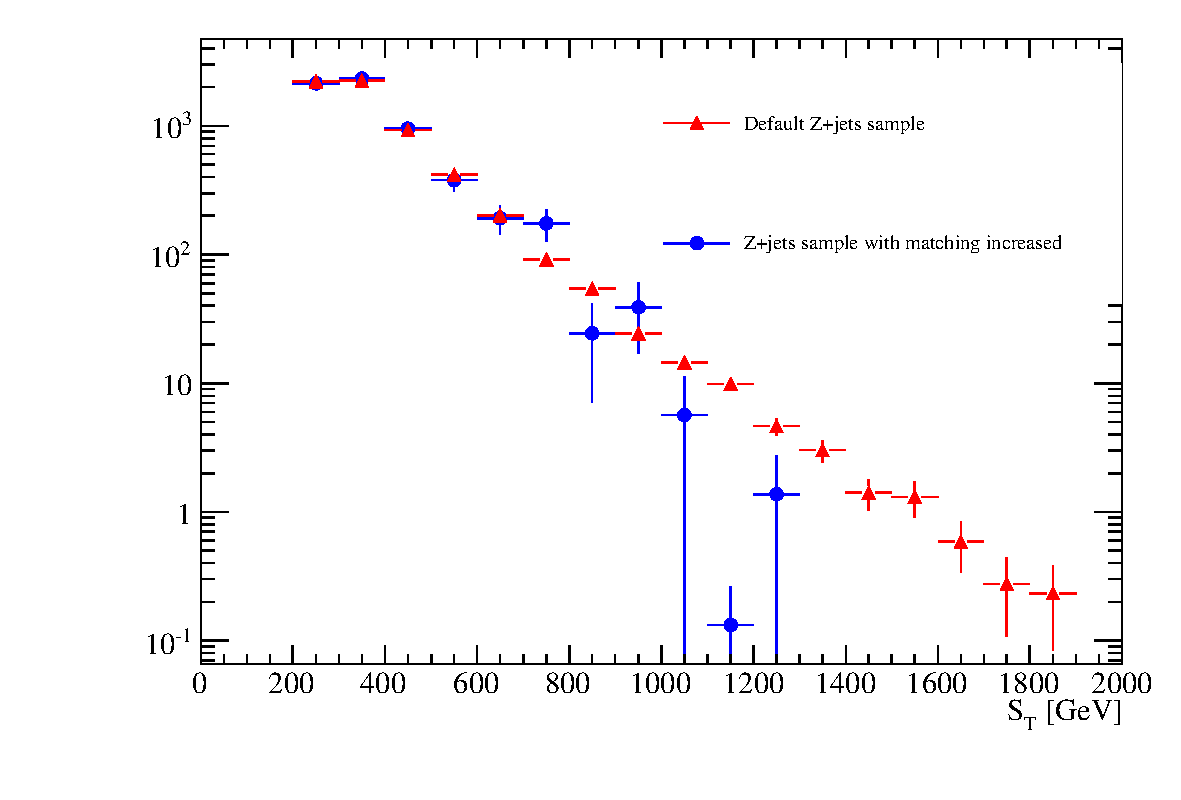
\includegraphics{tex/analysis/systematics/fig/MeePresel_MejPresel_STFinal_ZJetsToLL_matchingup_sT_PAS.pdf}} \\
      \resizebox{10cm}{!}{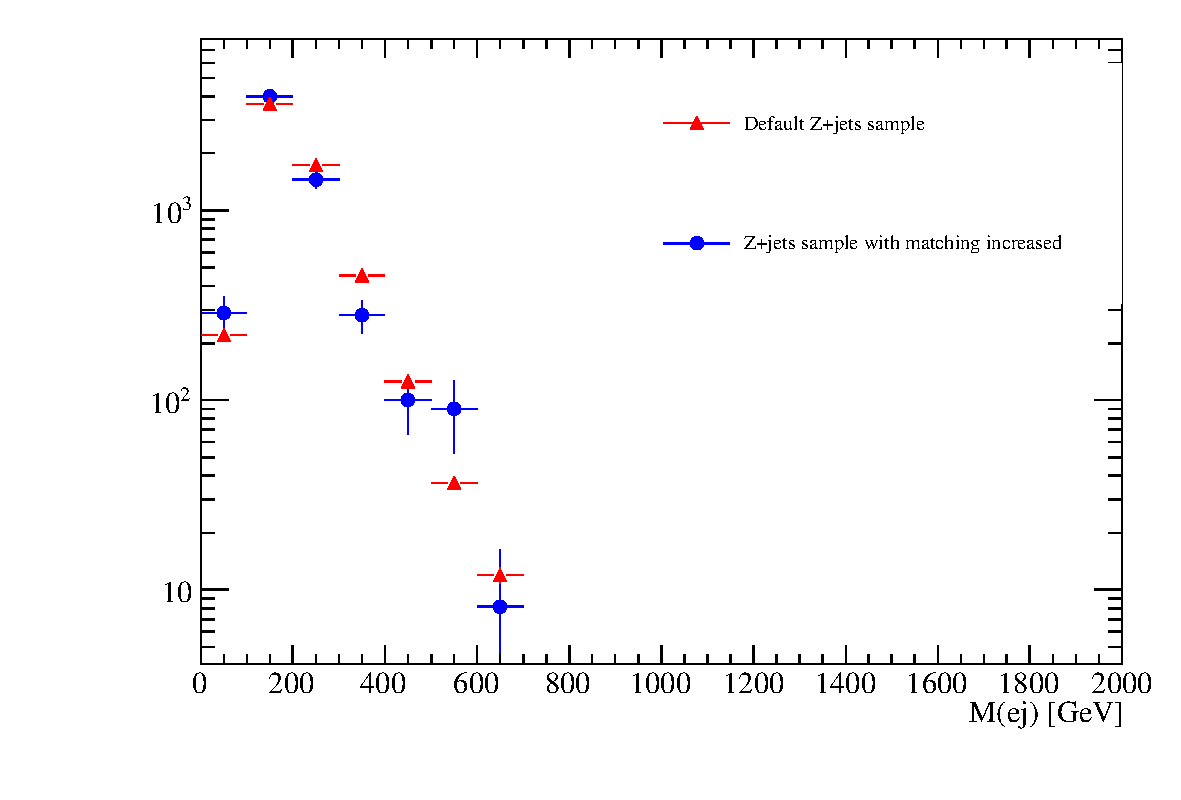
\includegraphics{tex/analysis/systematics/fig/MeePresel_MejFinal_STPresel_ZJetsToLL_matchingup_Mej_selected_avg_PAS.pdf}} \\
    \end{tabular}
    \caption{Comparison of \mee, \st, and \mej~distributions 
    between default and alternative samples for \zjets~background shape studies in the \eejj~channel.
    The plots refer to the selection criteria reported in Table~\ref{tab:ResultsShapeSyst}.}
    \label{fig:ResultsShapeSystZJets}
  \end{center}
\end{figure}   

 \begin{figure}[htbp]
  \begin{center}
    \begin{tabular}{cc}
      \resizebox{10cm}{!}{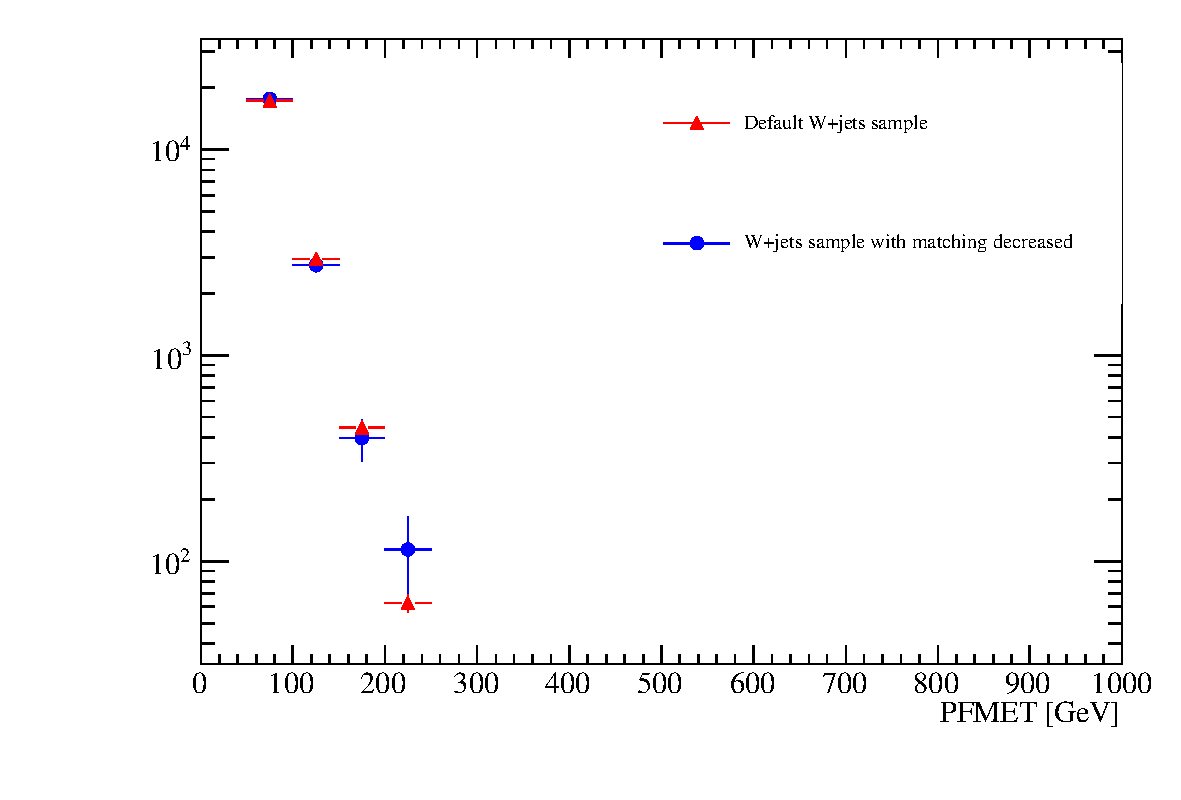
\includegraphics{tex/analysis/systematics/fig/METFinal_MejPresel_STPresel_WJetsToLNu_matchingdown_MET_PAS.pdf}} \\
      \resizebox{10cm}{!}{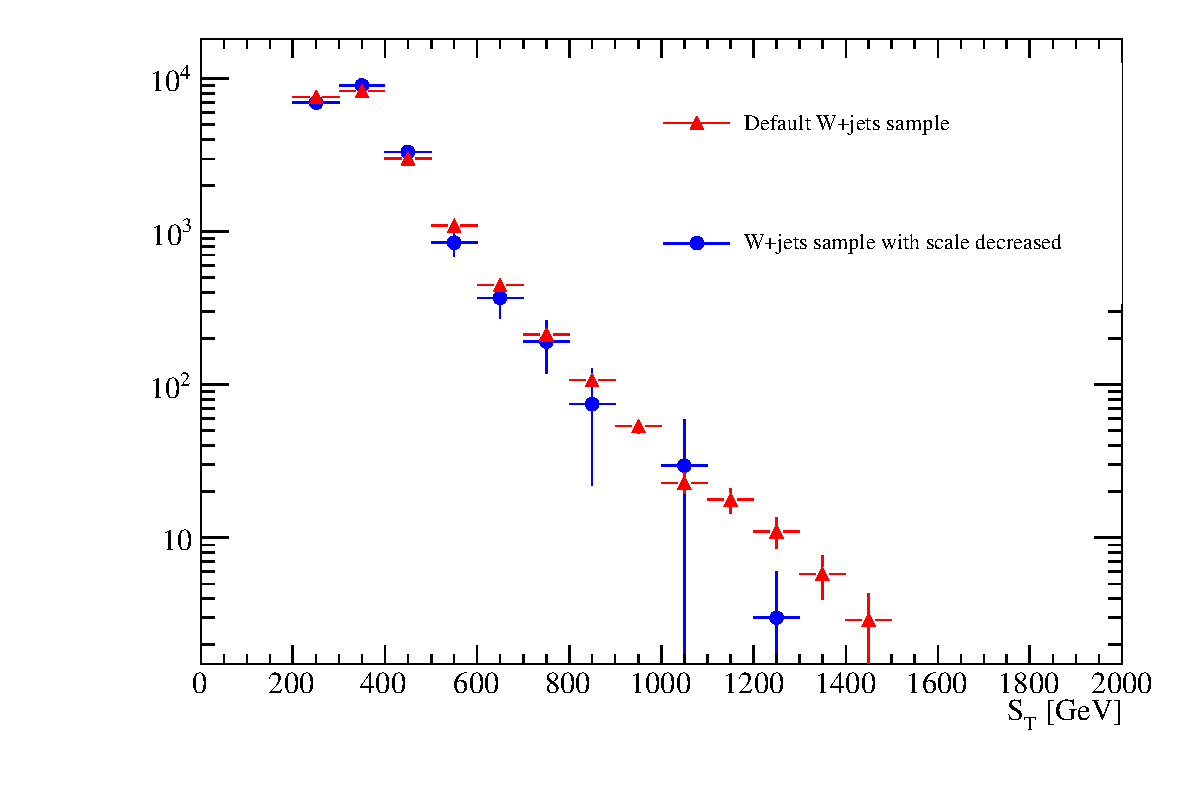
\includegraphics{tex/analysis/systematics/fig/METPresel_MejPresel_STFinal_WJetsToLNu_scaledown_sT_PAS.pdf}} \\
      \resizebox{10cm}{!}{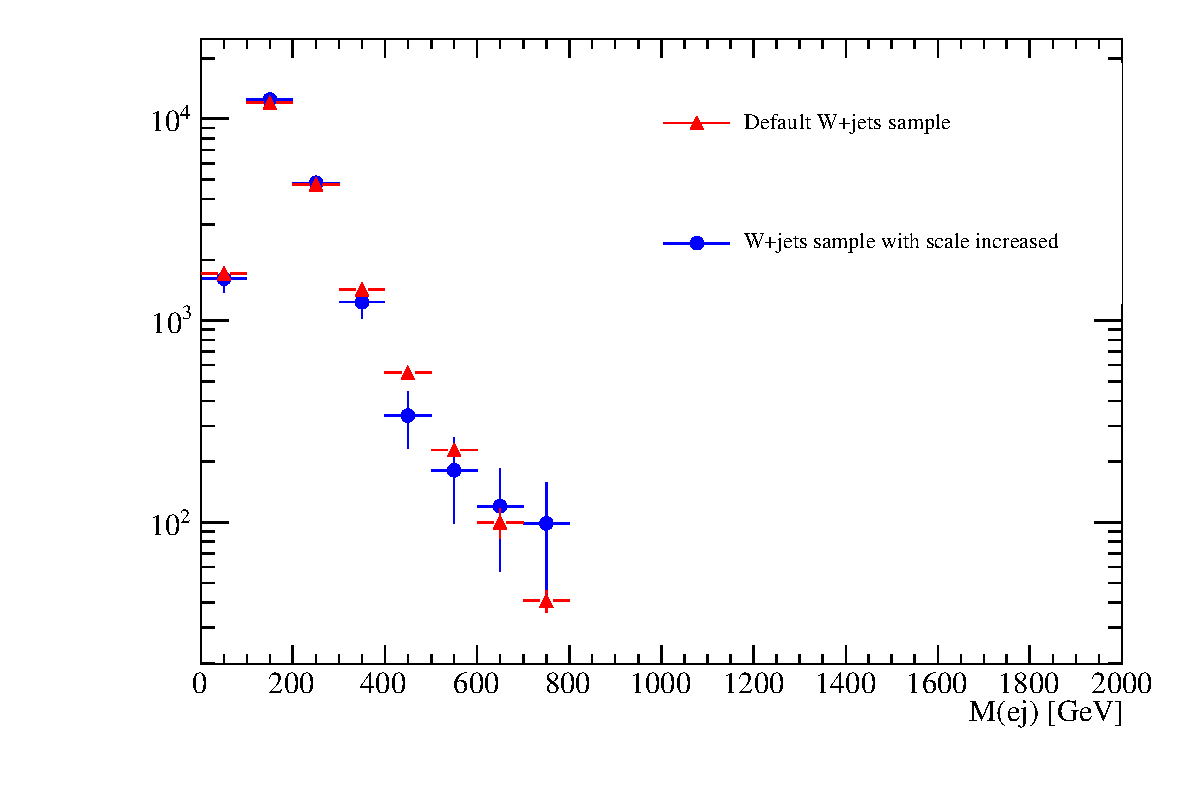
\includegraphics{tex/analysis/systematics/fig/METPresel_MejFinal_STPresel_WJetsToLNu_scaleup_Mej_PAS.pdf}} \\
    \end{tabular}
    \caption{Comparison of \MET, \st, and \mej~distributions 
    between default and alternative samples for \wjets~background shape studies in \enujj~channel.
    The plots refer to the selection criteria reported in Table~\ref{tab:ResultsShapeSyst}.}
    \label{fig:ResultsShapeSystWJets}
  \end{center}
\end{figure}   


 \begin{figure}[htbp]
  \begin{center}
    \begin{tabular}{cc}
      \resizebox{10cm}{!}{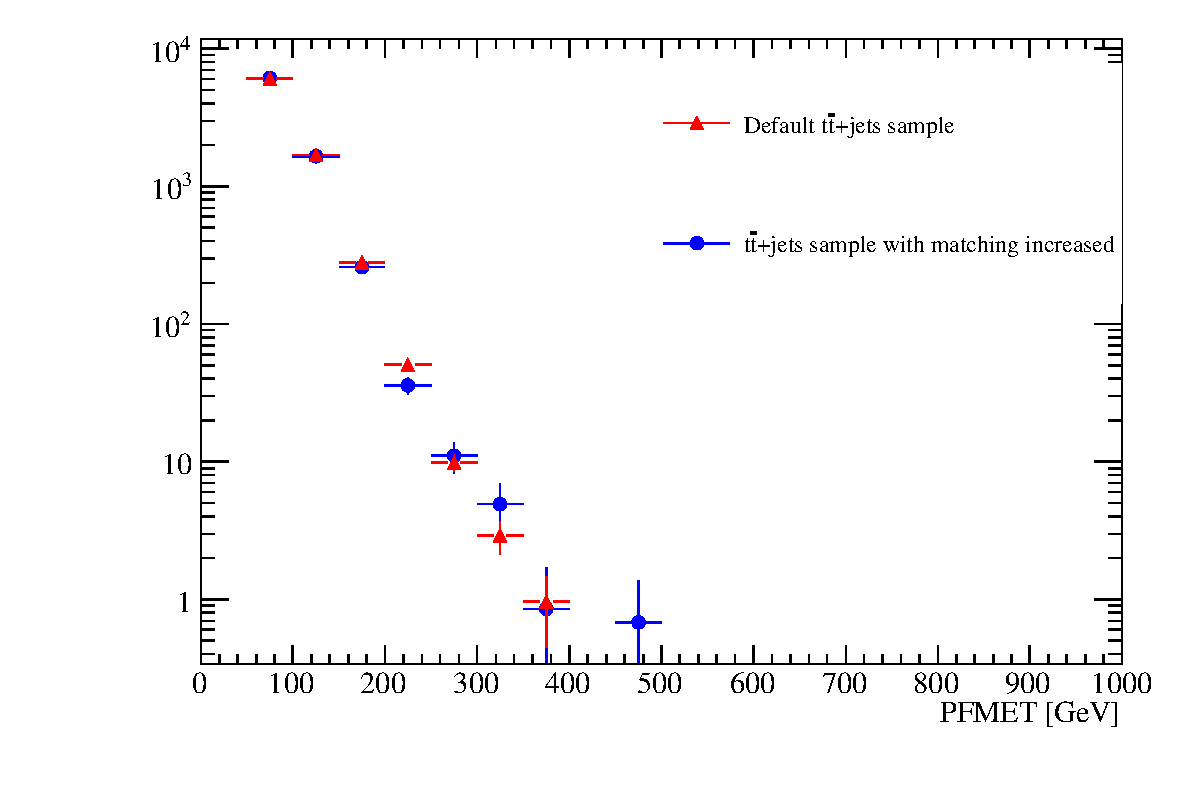
\includegraphics{tex/analysis/systematics/fig/METFinal_MejPresel_STPresel_TTjets_matchingup_MET_PAS.pdf}} \\
      \resizebox{10cm}{!}{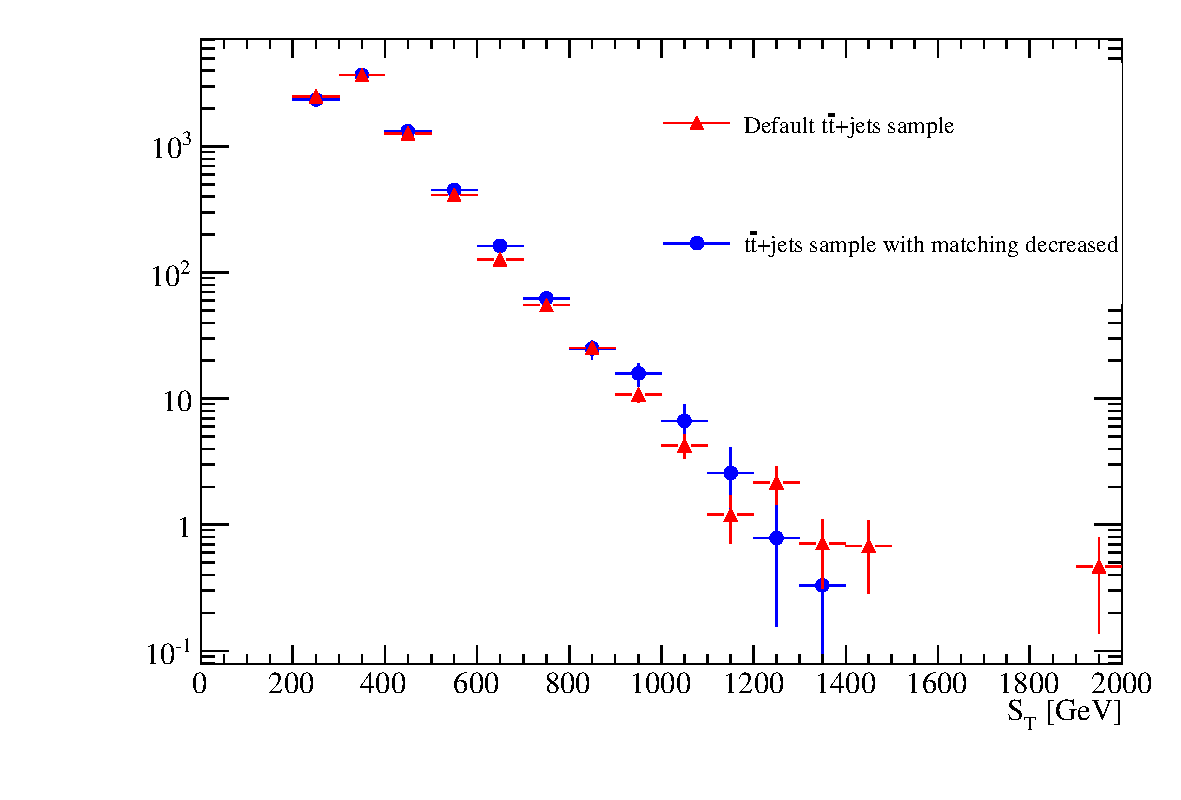
\includegraphics{tex/analysis/systematics/fig/METPresel_MejPresel_STFinal_TTjets_matchingdown_sT_PAS.pdf}} \\
      \resizebox{10cm}{!}{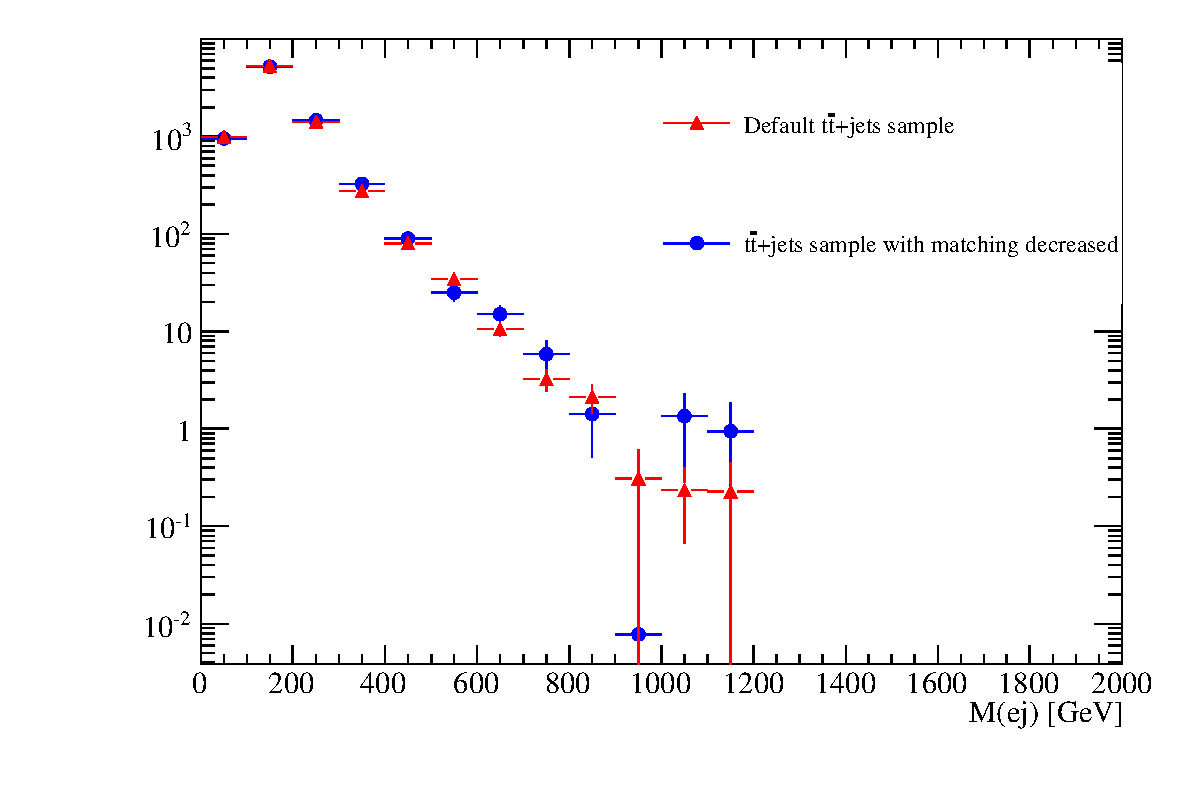
\includegraphics{tex/analysis/systematics/fig/METPresel_MejFinal_STPresel_TTjets_matchingdown_Mej_PAS.pdf}} \\
    \end{tabular}
    \caption{Comparison of \MET, \st, and \mej~distributions 
    between default and alternative samples for \ttbar~background shape studies in \enujj~channel.
    The plots refer to the selection criteria reported in Table~\ref{tab:ResultsShapeSyst}.}
    \label{fig:ResultsShapeSystTTbar}
  \end{center}
\end{figure}   


\section{Electron, jet, and \MET~energy scales}
\label{jetenergyscale}

The electron energy scale uncertainty in the EB 
(EE) is estimated to be \EESEB~(\EESEE) \cite{EES}.
A conservative \JES~uncertainty on the jet energy scale is used for the  
entire $\eta$ and \pt~range of the reconstructed jets~\cite{JES}.
For the jet and electron energy scales, 
the event selection is repeated rescaling by $1 \pm \sigma$ the energy of the reconstructed 
objects, where $\sigma$ is the relative uncertainty on their energy scales. While the electron and jet energy scale 
uncertainties are independent, the \MET~scale is directly correlated with both electron and jet energy scales. 
Therefore, while varying the electron and jet energy scales, a new \MET~vector is computed event-by-event using
Equation \ref{eqn:met-syst}:
\begin{equation}
  \vec{\mbox{\MET}}' = \vec{\mbox{\MET}} + \sum_{\text{electrons OR jets}} (\vec{p_T}-\vec{p_T}') 
  \label{eqn:met-syst}
\end{equation} 
where $\vec{p_T}$ is the \pt~vector of the original electron/jet, 
$\vec{p_T}'$ is the \pt~vector of the electron/jet with modified energy scale, 
and the sum is performed over all the reconstructed electrons/jets with \pt$>$30~\GeV. 
The analysis is then repeated using both $\vec{p_T}'$ of electrons/jets 
and $\vec{\mbox{\MET}}'$ at the same time. 

For the backgrounds with data driven normalization, the same 
rescaling procedure adopted for the default MC sample is also repeated 
for the samples with varied electron and jet energy scales. 
This makes it possible to 
evaluate the impact of electron and jet energy scale systematic uncertainties
on the final selection relative to the preselection stage.
In order to protect against statistical fluctuations
while calculating these systematic uncertainties, 
a maximum of 10\% statistical uncertainty on the number of MC events passing the final selection
is required for each systematic uncertainty measurement.
When the number of MC events becomes too small (with increasing mass on LQ hypothesis) 
the impact of the systematic uncertainty for a given selection is estimated to be the same as the 
impact of the systematic uncertainty corresponding to the selection of the 
highest mass point satisfying the 10\% condition.

At each stage of the final selection, 
the greatest magnitude of relative change in the number of signal and 
background events due to the variations 
of the jet or electron energy scales is used to 
assess the (symmetric) systematic uncertainties. 

These uncertainties are not considered for the QCD multijet background in 
either the \eejj~or \enujj~channels, nor is it considered for the \ttbar~background in the \eejj~channel, 
since for those both the background shape and normalization are already 
derived from data.

\section{Electron and jet energy resolution}
\label{sec:jetresolution}

The effect of the jet energy resolution uncertainty in MC is calculated
by matching jets directly from the MC generator to jets that have been reconstructed 
by the CMS reconstruction algorithms.  The \pt~of the matched reconstructed jet is then reassigned
according to Equation \ref{eqn:jetresolution}:
\begin{equation}
\label{eqn:jetresolution}
p_{T, \text{RECO}}^{'} = p_{T, GEN} + c \cdot (p_{T, \text{RECO}} - p_{T, \text{GEN}})
\end{equation}
where $c$ is the ratio of the jet energy resolution in data vs. MC. This ratio
has been found to depend on the reconstructed jet's pseudorapidity, and the values for various pseudorapidity regions are shown in Table 
\ref{tab:jetresolution}.  No change is made to the \pt~of reconstructed jets for which no generator 
match can be made.  All of the changes to the reconstructed jet \pt~are propagated to the \MET, using 
Equation \ref{eqn:met-syst}, as discussed in the previous section.

\begin{table}
  \begin{center}
    \begin{tabular}{c|c}
      $|\eta|$ range & Data/MC Ratio  \\ 
      \hline \hline
      0.0 - 0.5 & 1.052 $\pm$ 0.012 (stat) $\pm$ 0.062 (syst)\\
      0.5 - 1.1 & 1.057 $\pm$ 0.012 (stat) $\pm$ 0.056 (syst)\\
      1.1 - 1.7 & 1.096 $\pm$ 0.017 (stat) $\pm$ 0.063 (syst)\\
      1.7 - 2.3 & 1.134 $\pm$ 0.035 (stat) $\pm$ 0.087 (syst)\\
      2.3 - 5.0 & 1.288 $\pm$ 0.127 (stat) $\pm$ 0.155 (syst)\\
    \end{tabular}
    \caption{Ratio between data and MC values for jet energy resolution for different pseudorapity regions of the detector, as measured by the CMS JetMET group}
    \label{tab:jetresolution}
  \end{center}
\end{table}

For the backgrounds with data driven normalization, the same 
rescaling procedure adopted for the default MC sample is also repeated 
for the samples with varied electron and jet energy scales. 
This makes it possible to 
evaluate the impact of electron and jet energy scale systematic uncertainties
on the final selection relative to the preselection stage.
In order to protect against statistical fluctuations
while calculating these systematic uncertainties, 
a maximum of 10\% statistical uncertainty on the number of MC events passing the final selection
is required for each systematic uncertainty measurement.
When the number of MC events becomes too small (with increasing mass on LQ hypothesis) 
the impact of the systematic uncertainty for a given selection is estimated to be the same as the 
impact of the systematic uncertainty corresponding to the selection of the 
highest mass point satisfying the 10\% condition.

At each stage of the final selection, 
the greatest magnitude of relative change in the number of signal and 
background events due to the variations 
of the jet or electron energy scales is used to 
assess the (symmetric) systematic uncertainties. 

The effect of the electron energy resolution uncertainty in MC is calculated
using the same method as for jets, but the value for $c$ is taken to be \EEREB~for electrons
in the barrel and \EEREE~for electrons in the endcap \cite{EES}.  
All of the changes to electron \pt~are propagated to the \MET.


These uncertainties are not considered for the QCD multijet background in 
either the \eejj~or \enujj~channels, nor is it considered for the \ttbar~background in the \eejj~channel, 
since for those both the background shape and normalization are already 
derived from data.


\section{Integrated luminosity}

The uncertainty on the luminosity is 2.2\% \cite{cms-lumi-uncertainty}, as discussed in Section \ref{sec:lumi}.

\section{MC statistics}
The statistical uncertainty on the number of MC events is summarized
after the full \eejj~(\enujj) event selection in Table~\ref{tab:eejjFinalSelection} 
(Table~\ref{tab:enujjFinalSelection} or Table~\ref{tab:enujjFinalSelection_Nov30}) for signal and background samples.
This is the dominant systematic uncertainty for both the \enujj~and \eejj~channels.

\section{Electron trigger, reconstruction, identification and isolation uncertainties}  \label{sec:EleHLTIDIsoUncer}

For the \eejj~channel, the trigger efficiency is assumed to be 100\% with negligible uncertainty, 
as described in Section~\ref{sec:eejjTrigger}.
For the \enujj~channel, a combination of single-electron and electron$+$\MET$+$dijets 
triggers are used depending on the data taking period: 
the efficiency with which the \enujj~trigger fires on events passing the electron, \met,
and jet-related cuts of the \enujj~preselection is measured to be 95.5$^{+1.0\%}_{-3.5\%}$, as 
described in Section~\ref{sec:enujjTrigger}.

The efficiency with which electrons from \PZz decays are 
reconstructed and pass the HEEP ID requirements have been
studied in the context of the Z'$\rightarrow \mbox{ee}$ 
analysis~\cite{zprime-2011}.
An overall uncertainty of 1.5\% on the single electron efficiency is used in this analysis. 

The trigger uncertainty and the reconstruction and identification uncertainties are summed in quadrature 
giving a total 3\% ($^{+2.0\%}_{-4\%}$) contribution to the 
uncertainty on the signal selection efficiency for the \eejj~(\enujj) channel.
A conservative value of $\pm$4\% is quoted for  the \enujj~channel.
For those background estimations where data-driven uncertainties have 
already been determined, these uncertainties are not considered.

\section{Parton distribution function (PDF)} 
Uncertainties due to the choice of parton distribution functions (PDF) of the proton lead to changes 
in the total cross section and the selection efficiencies for both signal and background processes. 
The effect of the PDF uncertainties on the signal acceptance amounts to less than 1\%.
For those background estimations where data-driven uncertainties have 
already been determined, these uncertainties are not considered.

\section{Pile-up} 
\label{sec:pile-up-uncertainty}
All MC events in this analysis are reweighted 
to represent the pile-up conditions observed in data (see Section \ref{sec:reco-gen}).
This reweighting assumes a value of the inelastic $pp$ interaction
cross section, which has an associated uncertainty of 8.5\%.
The MC is reweighted after varying this cross section up and down by 8.5\%,
and the analysis is repeated.
The number of events passing the full selection is calculated 
for the $\pm$10\% cases and the default one. 
The maximum variation with respect to the default is used to assess a systematic uncertainty.
The uncertainty is less than 1\% for leptoquark signal at all masses in both \eejj~and \enujj~channels.
For backgrounds, the uncertainty is less than 1\% (3\%) in the \eejj~(\enujj) channels.

\begin{table}
  \begin{center}
    \small
    \begin{tabular}{c|c|c|c} 
      Systematic  & Magnitude  & Effect on  & Effect on \\
      Uncertainty &     [\%]           & Signal [\%]    & Background [\%] \\                   
      \hline\hline
      Background Normalization &  Section~\ref{sec:BkgNormUncert} & -- &  2.5 \\
      Background Shape & Section~\ref{sec:BkgShapeUncert} & -- &  10.5 \\
      Jet Energy Scale $\star$ & 4 & 2 & 1 \\
      Electron Energy Scale Barrel (Endcap) $\star$ & 1(3) & 1 & 6 \\
      Jet Energy Resolution & Section~\ref{sec:jetresolution} & 0.5 & 0.5 \\
      Electron Energy Resolution Barrel (Endcap) & 1(3) & 0.5 & 1 \\
      Electron Trigger/Reco/ID/Iso Efficiency & Section~\ref{sec:EleHLTIDIsoUncer} & 3 & -- \\
      Pileup   & 8.5 & 1 & 1 \\  
      MC statistics & Table~\ref{tab:eejjFinalSelection} & 0.5 & 28 \\
      Integrated Luminosity & 2.2 & 2.2 & 0.5 \\
      \hline
      Total & & 4.5 & 30 \\
    \end{tabular}
    \caption{Systematic uncertainties for \eejj~channel relative to the selection optimized for a LQ mass of 500 \GeV. 
      Note $\star$: the jet and electron energy scale uncertainties are also propagated to the \MET~calculation.}
    \label{tab:eejjSystematics}    
  \end{center}
\end{table}

\begin{table}
  \begin{center}
    \small
    \begin{tabular}{c|c|c|c} 
      Systematic  & Magnitude  & Effect on      & Effect on \\
      Uncertainty &     [\%]           & Signal [\%]  & Background [\%] \\                   
      \hline\hline
      Background Normalization & Section~\ref{sec:BkgNormUncert} & -- &  7 \\
      Background Shape & Section~\ref{sec:BkgShapeUncert} & -- &  11 \\
      Jet Energy Scale $\star$ & 4 & 6 & 12 \\
      Electron Energy Scale Barrel (Endcap)  $\star$ & 1(3) & 1.5 & 4.5 \\
      Jet Energy Resolution & Section~\ref{sec:jetresolution}& 0.5 & 9 \\
      Electron Energy Resolution Barrel (Endcap) & 1(3) & < 0.5 & 1.5 \\
      Electron Trigger/Reco/ID/Iso Efficiency & Section~\ref{sec:EleHLTIDIsoUncer} & 4 & -- \\
      Pileup   & 8.5 & 1 & 2 \\  
      MC statistics & Table~\ref{tab:enujjFinalSelection} or ~\ref{tab:enujjFinalSelection_Nov30}  & 1.0 & 19 \\
      Integrated Luminosity & 2.2 & 2.2 & -- \\
      \hline
      Total & & 8 & 28 \\
    \end{tabular}
  \caption{Systematic uncertainties for \enujj~channel relative to the selection optimized 
    for a LQ mass of 500 \GeV. Note $\star$: the 
    jet and electron energy scale uncertainties are also propagated to the \MET~calculation.}
  \label{tab:enujjSystematics}
  \end{center}
\end{table}
